% #######################################
% ########### FILL THESE IN #############
% #######################################
\def\mytitle{Coursework Report}
\def\myauthor{Maria Luque Anguita}
\def\contact{40280156@napier.ac.uk}
\def\mymodule{Advanced Web Technologies (SET09103)}
% #######################################
% #### YOU DON'T NEED TO TOUCH BELOW ####
% #######################################
\documentclass[10pt, a4paper]{article}
\usepackage[a4paper,outer=1.5cm,inner=1.5cm,top=1.75cm,bottom=1.5cm]{geometry}
\twocolumn
\usepackage{graphicx}
\graphicspath{{./images/}}
%colour our links, remove weird boxes
\usepackage[colorlinks,linkcolor={black},citecolor={blue!80!black},urlcolor={blue!80!black}]{hyperref}
%Stop indentation on new paragraphs
\usepackage[parfill]{parskip}
%% Arial-like font
\usepackage{lmodern}
\renewcommand*\familydefault{\sfdefault}
%Napier logo top right
\usepackage{watermark}
%Lorem Ipusm dolor please don't leave any in you final report ;)
\usepackage{lipsum}
\usepackage{xcolor}
\usepackage{listings}
%give us the Capital H that we all know and love
\usepackage{float}
%tone down the line spacing after section titles
\usepackage{titlesec}
%Cool maths printing
\usepackage{amsmath}
%PseudoCode
\usepackage{algorithm2e}

\titlespacing{\subsection}{0pt}{\parskip}{-3pt}
\titlespacing{\subsubsection}{0pt}{\parskip}{-\parskip}
\titlespacing{\paragraph}{0pt}{\parskip}{\parskip}
\newcommand{\figuremacro}[5]{
    \begin{figure}[#1]
        \centering
        \includegraphics[width=#5\columnwidth]{#2}
        \caption[#3]{\textbf{#3}#4}
        \label{fig:#2}
    \end{figure}
}

\lstset{
	escapeinside={/*@}{@*/}, language=C++,
	basicstyle=\fontsize{8.5}{12}\selectfont,
	numbers=left,numbersep=2pt,xleftmargin=2pt,frame=tb,
    columns=fullflexible,showstringspaces=false,tabsize=4,
    keepspaces=true,showtabs=false,showspaces=false,
    backgroundcolor=\color{white}, morekeywords={inline,public,
    class,private,protected,struct},captionpos=t,lineskip=-0.4em,
	aboveskip=10pt, extendedchars=true, breaklines=true,
	prebreak = \raisebox{0ex}[0ex][0ex]{\ensuremath{\hookleftarrow}},
	keywordstyle=\color[rgb]{0,0,1},
	commentstyle=\color[rgb]{0.133,0.545,0.133},
	stringstyle=\color[rgb]{0.627,0.126,0.941}
}

\thiswatermark{\centering \put(336.5,-38.0){\includegraphics[scale=0.8]{logo}} }
\title{\mytitle}
\author{\myauthor\hspace{1em}\\\contact\\Edinburgh Napier University\hspace{0.5em}-\hspace{0.5em}\mymodule}
\date{}
\hypersetup{pdfauthor=\myauthor,pdftitle=\mytitle,pdfkeywords=\mykeywords}
\sloppy
% #######################################
% ########### START FROM HERE ###########
% #######################################
\begin{document}
	\maketitle
	\begin{abstract}
	    The aim of this coursework is to demonstrate my understanding of the Python Flask micro-framework by creating a prototype web application for an online directory about a given subject. The subject here is food, hence why the webpage's title is 'Realfooding' and encourages people to start eating healthier. Food can be divided in real food or ultra-processed food. My web page explains the difference between them and contains many recipes and meal plans depending on the user's lifestyle, where everything is linked to make sure that every ingredient is explained and shows its benefits and drawbacks. Users can also leave doubts or comments that the web owner can then read in the Contact area and answer them.
	\end{abstract}


	\section{Introduction}
	My Realfooding web-app starts with a clear and easy to navigate display where the user can choose what is it that they want to read about, or if they want to get in touch with the specialist. As we scroll down more options appear while the image is still to make it easier to read the options.

	\includegraphics[width=8cm]{index.jpg}

    \textbf{Figure 2 Navigation diagram}
    \vspace{2mm}

    From there, we can go to different pages:
    \begin{itemize}
        \item Real food: contains different options to read about, like fruit, vegetables, fish and meat and others. Within those pages, the user can go and find even more information about every specific product that appears. This part contains the base information that then can be accessed from other parts of the web-app, i.e. since it contains aliments, all other recipes and food explanations have links to the aliment here.
        \item Ultra processed products: has information about what they are, why they are bad for us and examples.
        \item Meal plan: this page is the most informative one, it contains options to see different healthy and easy recipe ideas for breakfast, lunch, dinner or snacks, as well as a list of all the recipes there are in the web.
        \item Grocery Shopping: If there is no junk food at home, no one will eat junk food. These grocery shopping lists help people get only what they need and not more. It is divided in 3 options: diet, to lose weight; sports, to gain weight with a specific diet accompanied by doing sports; and events, which contains ideas for recipes that you can use for parties, since parties are normally related with chocolate and many ultra-processed foods.
        \item Contact: this last part is used for users to contact the specialist for any doubts or comments. The specialist will then read them and reply to them.
    \end{itemize}


    \section{Design}

    The web is divided just like the hierarchy shows in Appendix 1. All the objects such as aliments, recipes and doubts are saved in Json files. The web will take you to either base aliments or to recipes, which also contain links to the aliments themselves used in the recipe.

    Before starting to code anything I read various articles about how a good webpage is structured, where I found this quote: "DESIGNING WEB SOFTWARE IS DIFFERENT THAN DESIGNING WEBSITES[1]". This amazing website told me what steps to follow to start designing both, my website design and its software.

    Firstly, I started by creating an application flow, the quickest possible route to allow the user to get where it wants to and all the possible routes and endpoints there would be. Finally, I took my idea from rough sketches to a polish interface and a very effective program.

    Explaining how and why your web-app is structured the way it is. This section should include a navigation map for the URL hierarchy of your web-app.

    \section{Enhancements}

    Describing the features that you would add or improve.

    \section{Critical Evaluation}
    This is about what you built and should explain the features of the web-app that
you feel work well, or work poorly, and why.
404 errors all managed
login works
doubts correctly saved to json file
json files make it easy to bring and use information

 excellent level of functionality, both in terms of the number of
features and their quality of implementation
 have effectively evaluated

    \section{Personal Evaluation}
    This is about how you perfomed. You should reflect upon what you learned,
the challenges you faced, the methods you used to overcome challenges, and how you feel you
performed.

    \section{References}
    If you have used additional resources then these should be cited. Please acknowledge all
sources of help and material. If there is anything included that was not written by you for this
module, then you should indicate that within this section

    Designing Web Applications

    [1] \url{http://nathanbarry.com/webapps/}

https://en.wikipedia.org/wiki/Fruit#Nutritional_value
https://www.healthline.com/nutrition/how-much-fruit-per-day
https://iplaybaby.com/whole-baby-resource/info/types-of-fruits/
https://www.vegetables.co.nz/vegetables-a-z/
https://www.quora.com/Why-do-we-need-to-eat-vegetables
http://www.carballeira.com/en/white-fish-or-blue-fish/
https://www.safefood.eu/Healthy-Eating/What-is-a-balanced-diet/The-Food-Pyramid/Breads,-cereals-and-potatoes.aspx
https://mindovermunch.com/2018/05/03/are-processed-foods-bad/
https://www.sproutright.com/blog/index.php/5-reasons-you-need-snacks/

    \section{Appendices}

    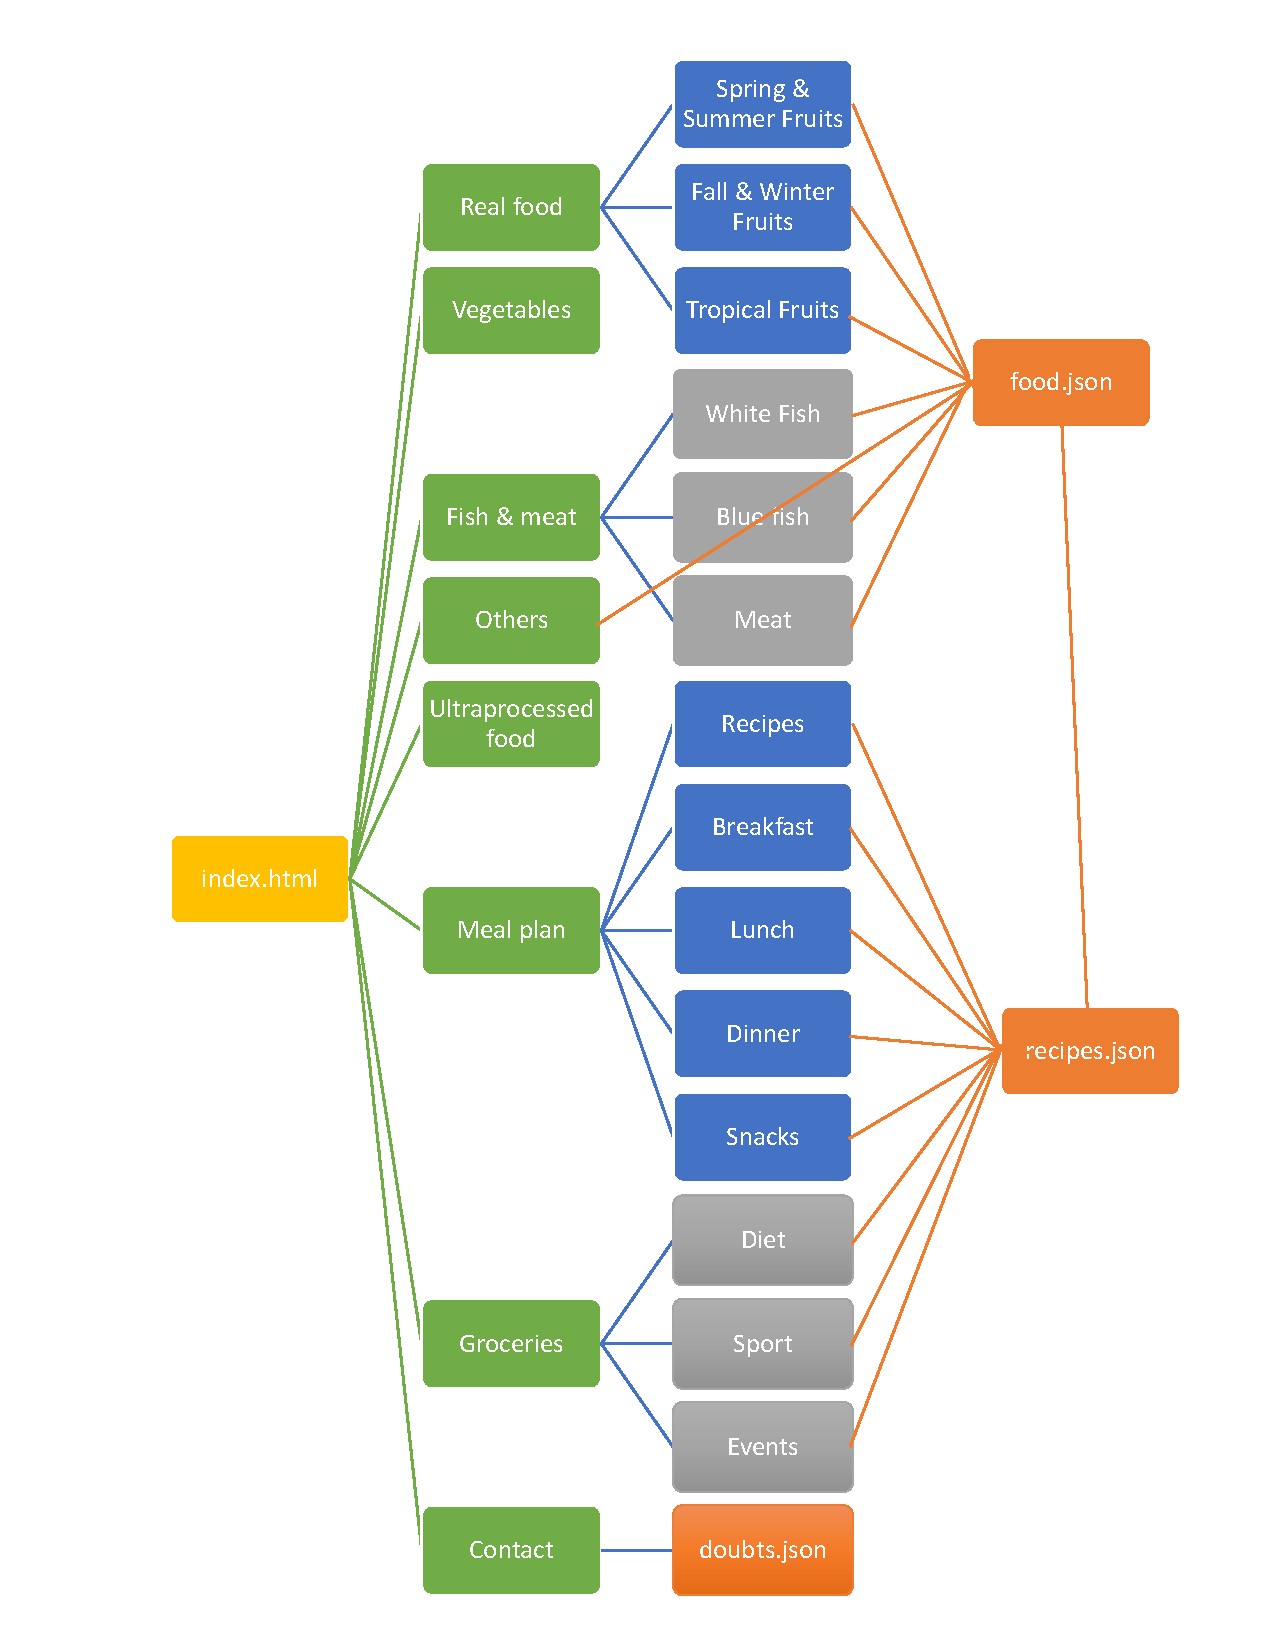
\includegraphics[width=8cm]{images/hierarchy.pdf}

    \textbf{Appendix 1 Navigation diagram}
    \vspace{2mm}

\end{document}
